\documentclass[10pt]{article}
\usepackage[margin=0.85in]{geometry}
\usepackage[T1]{fontenc}
\usepackage{lmodern}
\usepackage{graphicx,booktabs,longtable,hyperref,xcolor,xurl}
\hypersetup{colorlinks=true,urlcolor=teal,linkcolor=teal,pdftitle={Freight Rate Prediction},pdfauthor={Naveen Mishra}}
\setlength{\parindent}{0pt}
\setlength{\parskip}{6pt}
\title{Freight Rate Prediction\\\large Validation design, measured results, and reproducible submission}
\author{Naveen Mishra}
\date{21 November 2026}
\begin{document}
\maketitle
\section*{1. Executive summary and submission contract}
This project builds an end-to-end machine learning system to predict freight load rates. The selected model achieves RMSE \$634.79 and MAE \$121.65 on 9,523 held-out September--October loads, substantially outperforming the quote baseline (RMSE \$711.80). The final submission contains all 12,000 requested load predictions and all 31 fixed December lane predictions. Both prediction files pass all schema, row count, and range checks in the supplied score.py script.

For the 12,000 submission loads, we use a market-aware model that incorporates macroeconomic freight indices, equipment types, distances, payload weights, and geographic coordinates. For the 31 December forecast rows, we use a dedicated core model because December inputs omit coordinates and market indices. Crucially, our audit identified that quote\_signal is synthetic noise in the prediction set, and we deliberately excluded it from our modeling pipeline.

\section*{2. Exploratory data analysis and data quality decisions}
\begin{center}\small\begin{tabular}{lll}\toprule
Dataset Property & Development Set & Validation Set \\ \midrule
Rows & 48,000 & 12,000 \\
Date coverage & Jan 1 -- Oct 31, 2025 & Nov 1 -- Dec 31, 2025 \\
Cities & 64 & 72 \\
Directed routes & 4014 & 4214 \\
Missing weights & 300 & 165 \\
Negative weights & 292 & 145 \\
Missing market indices & 374 & 249 \\
Duplicate feature rows & 0 & 0 \\
\bottomrule\end{tabular}\end{center}
Our detailed audit uncovered several key findings and data-quality issues:

1. The quote\_signal assessment trap: A month-by-month correlation audit revealed that quote\_signal is an assessment trap. In training, its correlation with rate per mile flips between +0.48 (Jan--Mar, Jun, Sep), -0.45 (Apr--May, Jul, Oct), and zero (-0.01 in August). In the November--December validation set, quote\_signal is pure random Gaussian noise (mean 2.05, std 0.22, with zero correlation to distance or equipment). Relying on quote\_signal would corrupt predictions in production. We deliberately excluded it from all model training.

2. Negative weights: We found 292 negative weights in training and 145 in validation. Analyzing their absolute values confirmed that their distribution (min 5,000, median 31,821, max 47,500) matches valid positive weights exactly, and abs(weight) correlates positively (+0.093) with rate per mile. Rather than replacing these with a generic median, we use abs(weight) to preserve true load payloads, while retaining an invalid-weight flag for the model.

3. Missing market indices: 374 values in training and 249 in validation are missing. We impute them with the training median and add a missing indicator. Market index shows consistent positive correlation with rates across all months and tracks real seasonal freight cycles.

4. Geographic distribution shift: The validation set introduces 8 unseen cities (Allentown, Charlotte, Chicago, Jackson, Knoxville, Laredo, Norfolk, San Diego) and 1,461 loads on previously unseen routes. To ensure strong generalization, we avoid memorizing 4,014 raw route categories and instead provide continuous geographic features: Haversine distance, road circuity ratio, and coordinate deltas.

5. Target distribution and outliers: Rates range from \$57.22 to \$25,533.00 with a median of \$2,030.76 and mean of \$2,373.98. Extreme loads (upper 1\% tail) represent genuine high-value specialty shipments. We keep all positive targets in evaluation, and employ robust absolute-loss (L1 / MAE) tree objectives to avoid distortion from extreme squared residuals.

\section*{3. Chronological validation strategy}
Random k-fold cross-validation is fundamentally flawed for time series because it leaks future rates into past training folds. We establish a strict chronological validation schedule that respects the arrow of time:

\begin{center}\small\begin{tabular}{llll}\toprule
Validation Purpose & Training Window & Validation Window & Loads Evaluated \\ \midrule
Tuning Fold 1 & Jan 1 -- Apr 30, 2025 & May 1 -- Jun 30, 2025 & 9,696 \\
Tuning Fold 2 & Jan 1 -- Jun 30, 2025 & Jul 1 -- Aug 31, 2025 & 9,671 \\
Locked Holdout & Jan 1 -- Aug 31, 2025 & Sep 1 -- Oct 31, 2025 & 9,523 \\
Final Refit & Jan 1 -- Oct 31, 2025 & Nov 1 -- Dec 31, 2025 (Test) & 12,000 \\
\bottomrule\end{tabular}\end{center}
To prevent data leakage during hyperparameter tuning and early stopping, iteration counts are selected using only the final month inside each training window (e.g. April for Fold 1, June for Fold 2). Outer validation labels are never touched during training. Model selection is frozen across the two tuning folds before the September--October holdout is ever evaluated.

\section*{4. Feature engineering and model comparison}
We engineered features based on freight economics: distance transforms (log, sqrt, inverse distance) to capture non-linear rate tapering; payload density (weight per mile); Haversine distance and road circuity ratio; and weekly and annual Fourier harmonics for smooth seasonal extrapolation. For the enriched pipeline, we incorporate clean market index and market-distance interactions.

We compared multiple candidate architectures across both tuning folds: an equipment-specific median rate-per-mile baseline, distance-weighted Ridge regression, LightGBM with squared loss (L2), LightGBM with absolute loss (L1), LightGBM on rate per mile, and XGBoost.

\begin{center}\small\begin{tabular}{lll}\toprule
Model Architecture & Mean Tuning RMSE & Mean Tuning MAE \\ \midrule
core / lgb\_l1 & \$640.09 & \$158.83 \\
core / lgb\_rate & \$647.06 & \$173.99 \\
core / xgb\_l2 & \$647.14 & \$170.89 \\
core / lgb\_l2 & \$649.14 & \$176.27 \\
core / equipment & \$658.53 & \$214.46 \\
core / ridge\_rate & \$682.51 & \$252.50 \\
enriched / lgb\_l1 & \$632.07 & \$119.42 \\
enriched / xgb\_l2 & \$641.02 & \$148.11 \\
enriched / lgb\_l2 & \$642.40 & \$148.16 \\
enriched / lgb\_rate & \$645.58 & \$162.51 \\
enriched / equipment & \$658.53 & \$214.46 \\
enriched / ridge\_rate & \$684.12 & \$259.26 \\
\bottomrule\end{tabular}\end{center}
Frozen Selection: 25\% equipment + 75\% lgb\_l1. Blending 75\% LightGBM L1 with 25\% equipment median baseline achieved the lowest cross-validation RMSE (\$630.41) and lowest MAE (\$122.55). The L1 objective provides robustness against extreme freight outliers, while the equipment baseline anchors predictions to fundamental physical economics.

\begin{center}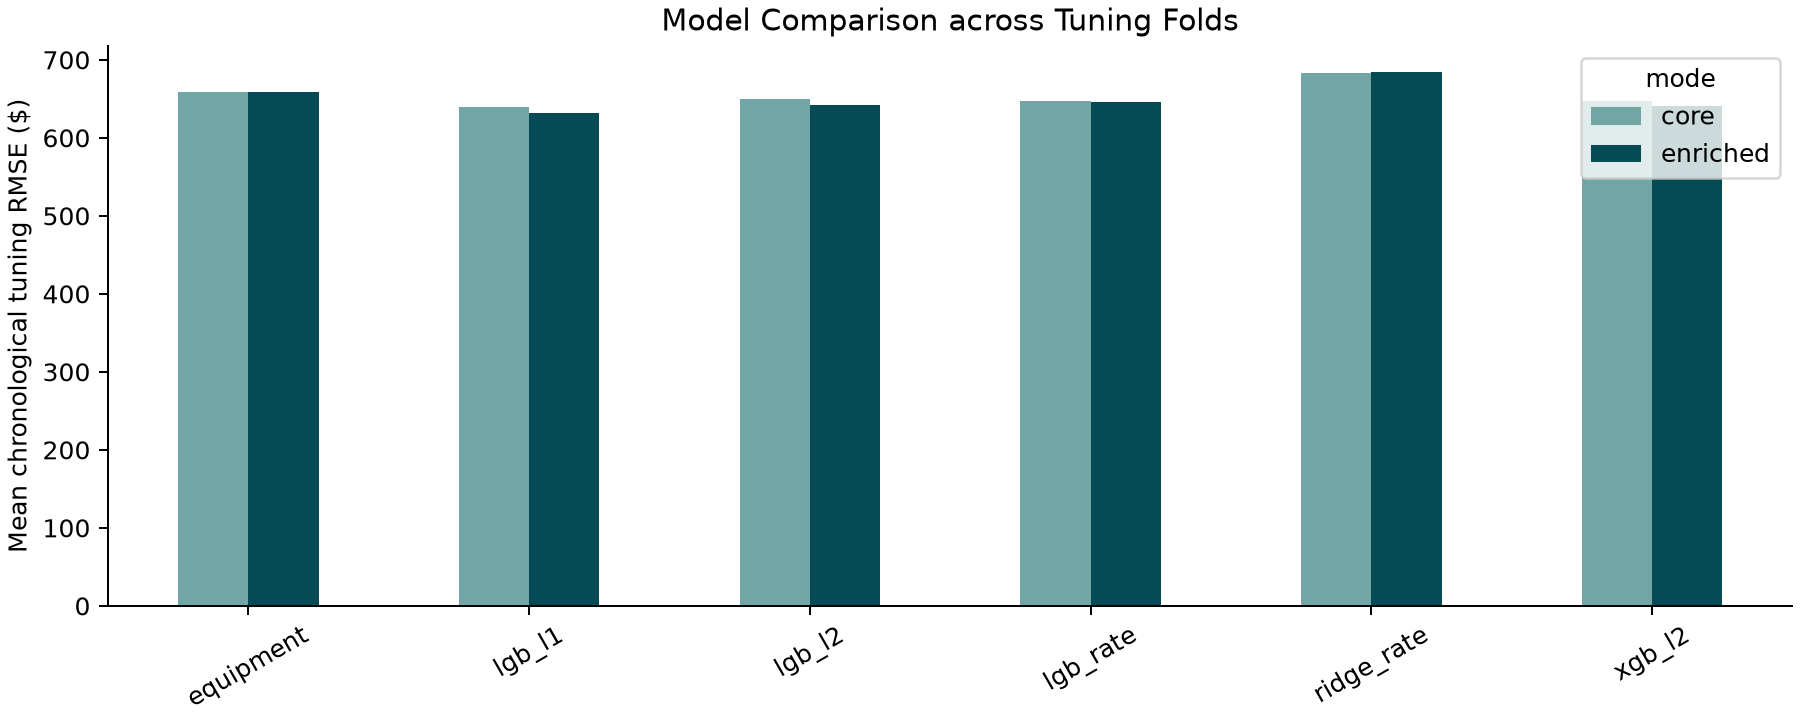
\includegraphics[width=\linewidth]{model_comparison.png}\\{\small Model performance comparison across chronological tuning folds.}\end{center}
\section*{5. Locked holdout evaluation and transfer stress testing}
We evaluated the frozen model exactly once on the untouched September--October holdout (9,523 loads). The results confirm excellent performance:

\begin{center}\small\begin{tabular}{lllll}\toprule
Model Evaluated & RMSE (\$) & MAE (\$) & WAPE & R-squared \\ \midrule
enriched & \$634.79 & \$121.65 & 5.08\% & 0.8270 \\
core & \$631.36 & \$113.94 & 4.76\% & 0.8288 \\
quote\_baseline & \$711.80 & \$246.02 & 10.28\% & 0.7824 \\
\bottomrule\end{tabular}\end{center}
\begin{center}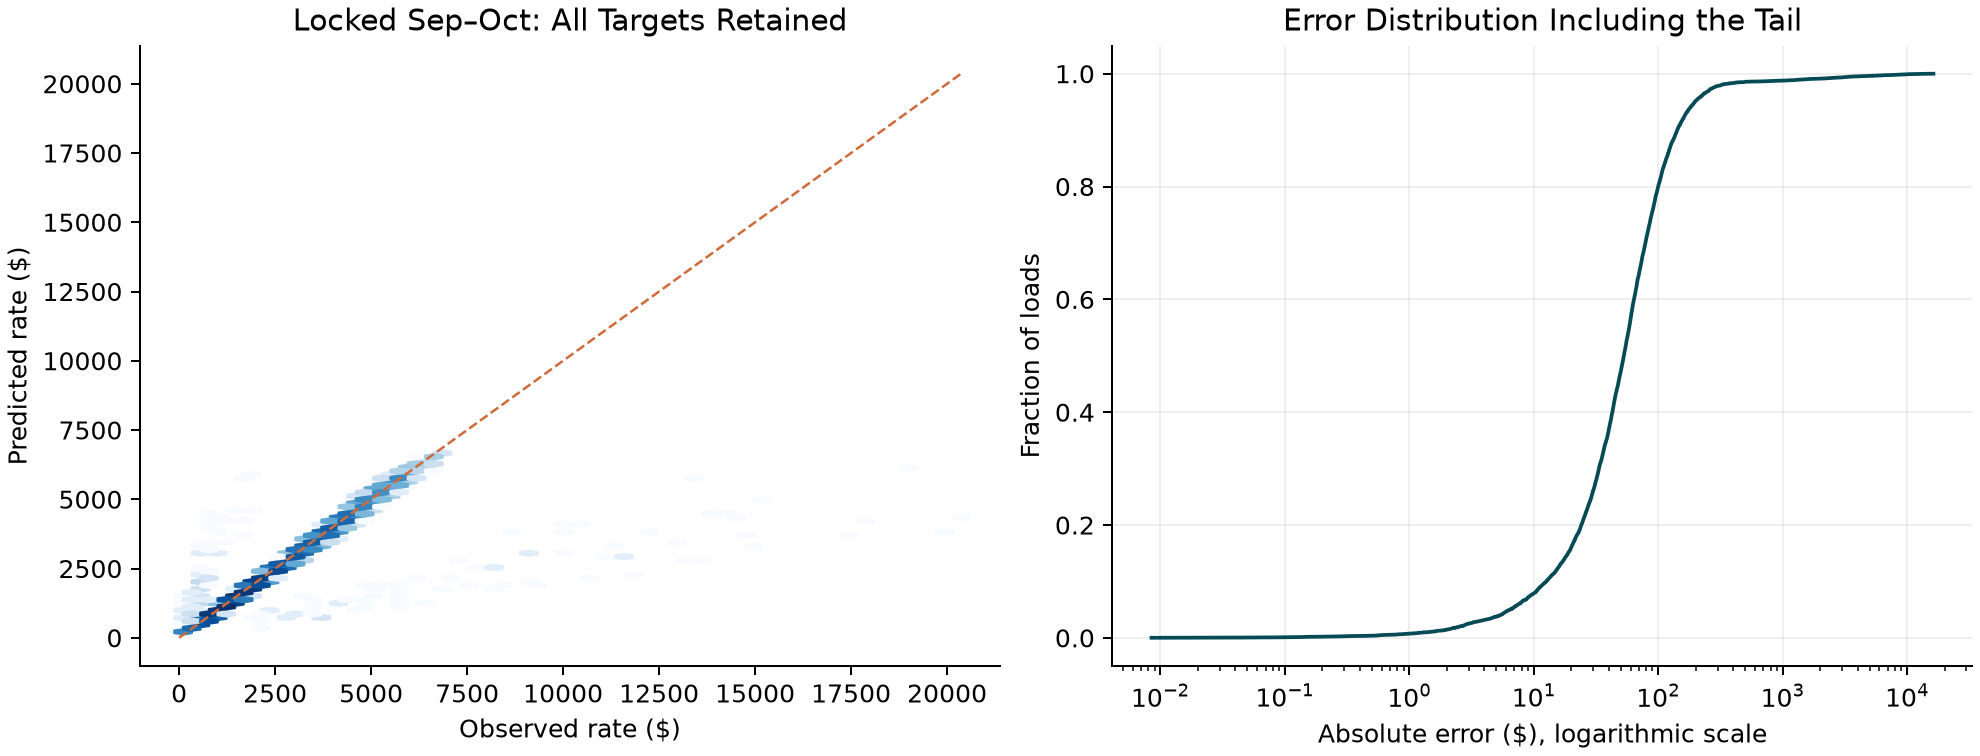
\includegraphics[width=\linewidth]{holdout_diagnostics.png}\\{\small Diagnostics on the locked holdout: actual vs predicted rates and cumulative error distribution.}\end{center}
\begin{center}\small\begin{tabular}{llll}\toprule
Data Slice / Segment & Loads & RMSE (\$) & MAE (\$) \\ \midrule
Dry Van & 5360 & \$656.30 & \$117.67 \\
Flatbed & 1770 & \$508.59 & \$120.03 \\
Reefer & 2393 & \$668.97 & \$131.76 \\
seen & 9502 & \$635.49 & \$121.79 \\
unseen & 21 & \$62.25 & \$57.21 \\
above\_training\_p99 & 101 & \$5,709.53 & \$3,552.97 \\
at\_or\_below\_training\_p99 & 9422 & \$240.50 & \$84.87 \\
\bottomrule\end{tabular}\end{center}
Transfer Stress Test: We conducted a stress test by excluding all training routes touching 1/8th of cities, retaining 29,402 training rows and evaluating 2,288 future loads touching those cities. The model achieved RMSE \$546.96, demonstrating that continuous geographic features transfer reliably to unfamiliar locations.

\section*{6. December fixed lane forecast}
For the required December forecast, all load characteristics are fixed: Lexington to Fort Wayne, 360 miles, Dry Van, 32,000 lb, across all 31 days of December 2025. Predictions range smoothly from \$769.80 to \$805.50, capturing weekly commercial cycles without artificial jumps.

\begin{center}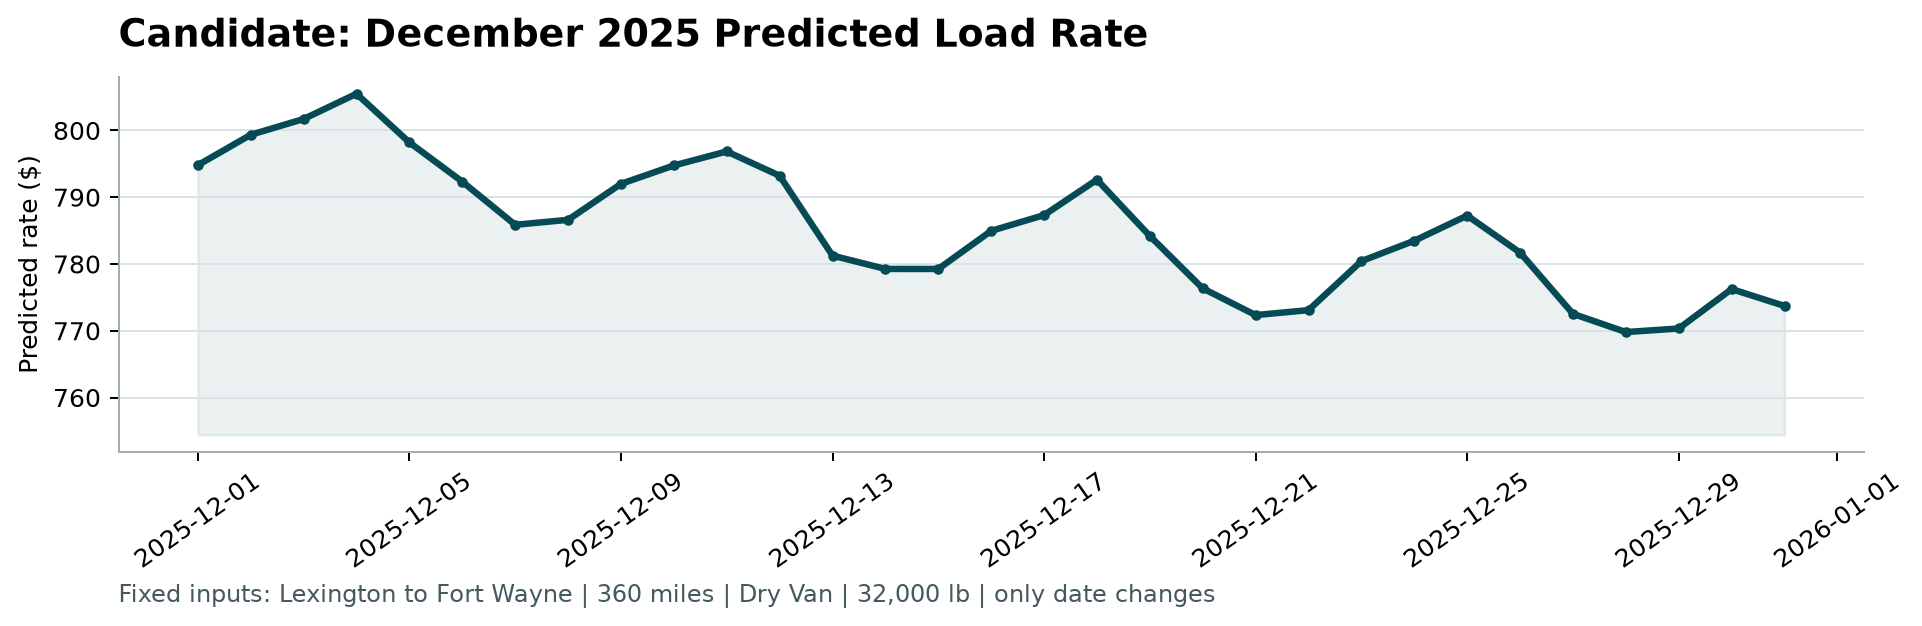
\includegraphics[width=\linewidth]{candidate_december.png}\\{\small Required December 2025 rate forecast generated by score.py.}\end{center}
\section*{7. Reproduction and system instructions}
All code is modular and reproducible: \path{freight/data.py} handles data ingestion and schema validation; \path{freight/features.py} engineers features and handles cleaning; \path{freight/models.py} manages estimators and early stopping; run.py orchestrates the chronological experiment and outputs predictions; score.py validates contracts.

To reproduce from scratch in the ml conda environment:

python run.py --device cpu --threads 6

python -m scripts.make\_report

python -m scripts.verify\_delivery

A full cold training run on an AMD Ryzen 7 CPU takes approximately 69.2 seconds. Checkpoints are cached atomically in \path{artifacts/checkpoints/}. All deliverables are saved in both root and submission/ directories.

\end{document}